\section{RSA} \label{sec:RSA}
%TODO	@farid complete this section

\subsection{MGF}
A mask generation function (MGF) is a cryptographic primitive similar to a cryptographic hash function except that while a hash function's output is a fixed size, a MGF supports output of a variable length. There may be restrictions on the length of the input and output octet strings, but such bounds are generally very largeMask generation functions are completely deterministic: for any given input and desired output length the output is always the same.
\subsubsection{MGF1}

MGF1 is a Mask Generation Function based on a hash function.
\\
\newline
\textbf{Algorithm overview}
\\
\newline
MGF1 (\textit{mgfSeed}, \textit{maskLen}): \\
\begin{table}[!h]
\begin{tabular}{lllll}
\textit{Options}: &  & Hash            & \begin{tabular}[c]{@{}l@{}}function (\textit{hLen} denotes the length \\ in octets of the hash function output)\end{tabular} &  \\
         &  &                 &                                                                                                                     &  \\
         &  &                 &                                                                                                                     &  \\
\textit{Input}:   &  & \textit{mgfSeed}         & seed from which mask is generated, an octet string                                                                  &  \\
         &  &                 &                                                                                                                     &  \\
         &  & \textit{maskLen}         & intended length in octets of the mask, at most  $2^{32}$ \textit{hLen}                                                             &  \\
         &  &                 &                                                                                                                     &  \\
         &  &                 &                                                                                                                     &  \\
\textit{Output}:  &  & \textit{mask}            & mask, an octet string of length \textit{maskLen}                                                                             &  \\
         &  &                 &                                                                                                                     &  \\
         &  &                 &                                                                                                                     &  \\
\textit{Error}:   &  & “mask too long” &                                                                                                                     & 
\end{tabular}
\end{table}

\textit{Steps}:
\newline
\begin{enumerate}
	\itemsep1em
	\item If $maskLen > 2^{32}\ hLen$, output “mask too long” and stop.
	\item Let \textit{T} be the empty octet string.
	\item For \textit{counter} from 0 to $\ceil{maskLen / hLen}$-1 , do the following:
	\begin{enumerate}[label=\Alph*.]
		\itemsep0.5em
		\item Convert counter to an octet string C of length 4 octets:\\ \newline C = I2OSP\footnote{You can find detail of the I2OSP function \cite{pkcs}.} (\textit{counter}, 4).
		\item Concatenate the hash of the seed \textit{mgfSeed} and \textit{C} to the octet string \textit{T}:\\ \newline $T = T || Hash (mgfSeed || C)$ .
	\end{enumerate}
	\item Output the leading \textit{maskLen} octets of \textit{T} as the octet string \textit{mask}.
\end{enumerate}
It is an example python code for MGF1. 
\newline
\begin{lstlisting}[language=Python, caption={MGF1 example on python}]
import hashlib

def i2osp(integer, size=4):
  return ''.join([chr((integer >> (8 * i)) & 0xFF) for i in
  	reversed(range(size))])

def mgf1(input, length, hash=hashlib.sha1):
  counter = 0
  output = ''
  while (len(output) < length):
    C = i2osp(counter, 4)
    output += hash(input + C).digest()
    counter += 1
  return output[:length]
\end{lstlisting}



\subsection{OAEP}
In cryptography, Optimal Asymmetric Encryption Padding \footnote{OAEP} is a padding scheme often used together with RSA encryption.
This processing is proved to result in a combined scheme which is semantically secure under chosen plaintext attack \footnote{IND-CPA}.

\subsubsection{Encryption operation}

RSAES-OAEP-ENCRYPT (($n$, $e$), $M$, $L$):

\begin{table}[!h]
\begin{tabular}{lllll}
Options:    &  & Hash   & \begin{tabular}[c]{@{}l@{}}hash function ($hLen$ denotes the length in octets of the hash\\ function output)\end{tabular}                                        &  \\
            &  &        &                                                                                                                                                                &  \\
            &  & MGF    & mask generation function                                                                                                                                       &  \\
            &  &        &                                                                                                                                                                &  \\
$Input$:      &  & ($n$, $e$) & \begin{tabular}[c]{@{}l@{}}recipient’s RSA public key ($k$ denotes the length in octets of the\\ RSA modulus $n$)\end{tabular}                                     &  \\
            &  &        &                                                                                                                                                                &  \\
            &  & M      & \begin{tabular}[c]{@{}l@{}}message to be encrypted, an octet string of length $mLen$, where\\ $mLen \leq k-2hLen-2$\end{tabular}                                  &  \\
            &  &        &                                                                                                                                                                &  \\
            &  & $L$      & \begin{tabular}[c]{@{}l@{}}optional label to be associated with the message; the default value\\ for $L$, if $L$ is not provided, is the empty string\end{tabular} &  \\
            &  &        &                                                                                                                                                                &  \\
            &  &        &                                                                                                                                                                &  \\
$Output$:     &  & $C$      & ciphertext, an octet string of length $k$                                                                                                                        &  \\
            &  &        &                                                                                                                                                                &  \\
            &  &        &                                                                                                                                                                &  \\
$Error$:      &  &        & “message too long”; “label too long”                                                                                                                           &  \\
            &  &        &                                                                                                                                                                &  \\
            &  &        &                                                                                                                                                                &  \\
$Assumption$: &  &        & RSA public key ($n$, $e$) is valid                                                                                                                                 & 
\end{tabular}
\end{table}

\textit{Steps}:
\newline
\begin{enumerate}
	\itemsep2em
	\item $Length checking$:
	\begin{enumerate}[label=\alph*.]
		\itemsep1em
		\item If the length of L is greater than the input limitation for the hash function ($2^{61}-1$ octets for SHA-1), output “label too long” and stop.
		\item If $mLen > k-2hLen-2$, output “message too long” and stop.
	\end{enumerate}
	\item $EME-OAEP encoding$ (see Figure \ref{fig:RSA_OAEP} below):
	\begin{enumerate}[label=\alph*.]
		\itemsep1em
		\item If the label $L$ is not provided, let $L$ be the empty string. Let $lHash$ = Hash ($L$), an octet string of length $hLen$.
		\item Generate an octet string PS consisting of $k - mLen - hLen - 2$ zero octets. The length of PS may be zero.
		\item Concatenate $lHash$, $PS$, a single octet with hexadecimal value $0x01$, and the message $M$ to form a data block $DB$ of length $k - hLen - 1$ octets as:\\
		\newline
		$DB = lHash\ ||\ PS\ ||\ 0x01\ ||\ M$.
		\item Generate a random octet string $seed$ of length $hLen$.
		\item Let $dbMask$ = MGF ($seed$, $k-hLen-1$)
		\item Let $maskedDB$ = $DB \oplus dbMask$.
		\item Let $seedMask$ = MGF ($maskedDB$, $hLen$).
		\item Let maskedSeed = $seed \oplus seedMask$.
		\item Concatenate a single octet with hexadecimal value $0x00$, maskedSeed, and $maskedDB$ to form an encoded message $EM$ of length $k$ octets as:\\
		\newline
		$EM = 0x00\ ||\ maskedSeed\ ||\ maskedDB$.
	\end{enumerate}
	\item $RSA encryption$:
	\begin{enumerate}[label=\alph*.]
		\itemsep1em
		\item Convert the encoded message EM to an integer message representative m:\\
		\newline
		$m$ = OS2IP($EM$) .
		\item Apply the RSAEP encryption primitive\footnote{Section 5.1.1 of \cite{pkcs}} to the RSA public key ($n$, $e$) and the message representative $m$ to produce an integer ciphertext representative c:\\
		\newline
		$c$ = RSAEP(($n$,$e$),$m$)
		\item Convert the ciphertext representative $c$ to a ciphertext $C$ of length $k$ octets:\\
		\newline
		$C$ = I2OSP($c$,$k$).
	
	\end{enumerate}
	\item Output the ciphertext $C$.
\end{enumerate}

\begin{figure}[!h]
\centering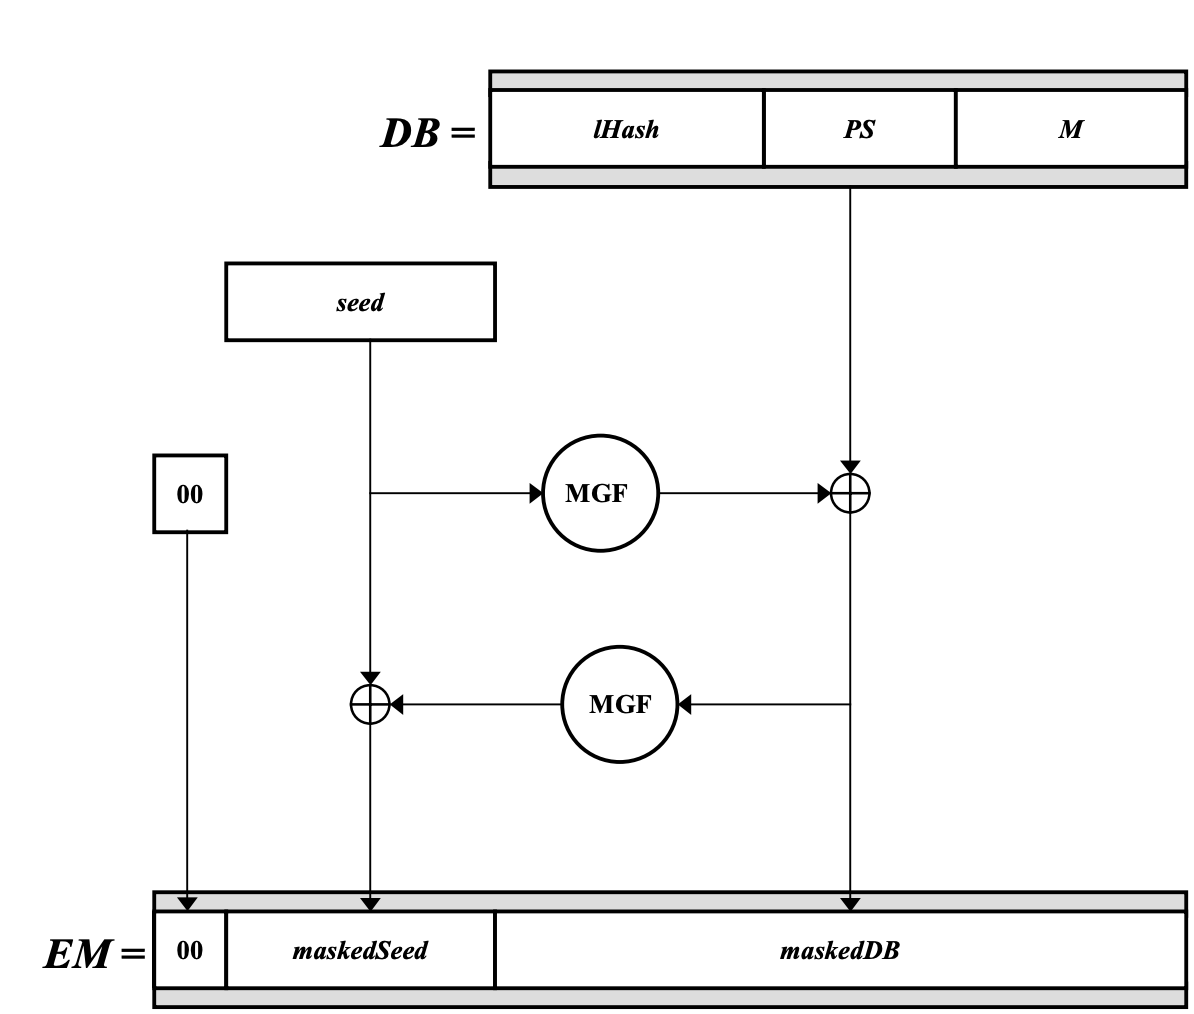
\includegraphics[scale=0.35]{EME-OAEP}
\caption{$lHash$ is the hash of the optional label $L$.
Decoding operation follows reverse steps to recover $M$ and verify $lHash$ and $PS$.}
\label{fig:RSA_OAEP} 
\end{figure}


Note. If $L$ is the empty string, the corresponding hash value $lHash$ has the following hexadecimal representation for SHA-1 Hash:\\

\begin{myfont}
	
\textbf{(0x)da39a3ee\ \ \ \ 5e6b4b0d\ \ \ \ 3255bfef\ \ \ \ 95601890\ \ \ \ afd80709}

\end{myfont}
















